\begin{frame}{Symmetry Protection of Degenerate Edge}
\vskip-1.5cm
  $$
    \ket{\psi} = \sum\limits_i \lambda_i \ket{\psi_L^i} \ket{\psi_R^i}
  $$
  \only<1>{
  \begin{columns}[T]
    \begin{column}{0.5\textwidth}
    
    Inversion symmetry $\mathcal{I}$ induces an antiunitary action $V_{\mathcal{I}} \kappa$ on the edge. 

    This occurs in two steps:
    \bi
    \item $\ket{e, K}_L \rightarrow \ket{e, -K}_R$
    \item $\ket{e, K}_R \rightarrow \ket{-e, -K}_L$
    \ei

    Combined:
    \bi
    \item[] $ V_{\mathcal{I}} \ket{e, K} \propto \ket{-e, K}$
    \ei
  
  Phases work out like this:
  $$ V_{\mathcal{I}} \sim \sigma_x = \begin{matrix}
  0 & 1 \\
  1 & 0
 \end{matrix} $$

 \end{column}
    
    \begin{column}{0.5\textwidth}
     Charge symmetry $\mathcal{\theta}$ induces a unitary action $V_{\mathcal{\theta}}$ on the edge. 

     Charge parity $\mathcal{\pi} \in U(1)$ induces the action 

     \bi
     \item[] $V_{\mathcal{\pi}}$ \ket{e, K} = (-1)^e \ket{e, K} 
     \ei

    $$ V_{\mathcal{\pi}} \sim \sigma_z = \begin{matrix}
  1 & 0 \\
  0 & -1
 \end{matrix} $$
 \end{column}
\end{columns}

\begin{center}
Combined antiunitary action $V_{\mathcal{I \pi}} \kappa $ satsfies

$$
V_{\mathcal{I \pi}} V_{\mathcal{I \pi}}^* = -1
$$
\end{center}

\end{frame}

% \begin{block}{1D Symmetry Protection}
%       \bi
%       \only<1>{
%       \item[] On-site symmetries $g$ come with projective representation $V_g$
%       \item $V_g$ acts on sets of degenerate Schmidt states
%       \item Charge and translation represented linearly on edge
%       }
%       \only<2>{
%       \item[] Time reversal symmetry $\tau$ represented by antiunitary    $V_{\tau} K$ on the edge
%       \item $\tau^2 = +1$ on this edge
%       }
%       \only<3>{
%       \item[] Inversion $\mathcal{I}$
%       \item  $\mathcal{I}$ in combination with swapping Schmidt states represented by antiunitary operation $V_{\mathcal{I}} K$ on the edge
%       \item $\mathcal{I}^2 = V_{\mathcal{I}} V_{\mathcal{I}}^{*} = 1$
      
%       \item[] Inversion $\mathcal{I}$ combined with $\mathcal{\pi} = e^{i\pi N}$
%       \item  $\mathcal{\pi I}$ represented antiunitarily on the edge
%        by $V_{\mathcal{\pi I}} K$
%       \item $(\mathcal{\pi I})^2 = 1$ but $V_{\mathcal{\pi I}} 
%       V_{\mathcal{\pi I}}^{*} = -1$
%       }
%       \ei
%     \end{block}
%     \end{column}
%     \begin{column}[T]{.4\textwidth}
%       \vskip2cm
%       \begin{figure}
%         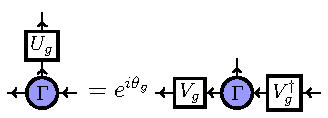
\includegraphics[width=\textwidth]{group_sym.pdf}